%
% The standard LaTeX article class is close to what is needed for an MPhys project report
\documentclass[12pt]{article}

% The following package makes the necessary tweaks to comply with the formatting requirements.
% It also provides a standardised title page, and will warn you if the main text is too long.
\usepackage{mphysproject}
\usepackage{tikz}
\usetikzlibrary{shapes,arrows,calc,math}
%
%% DO NOT GO CHANGING THE FONT SIZE OR MARGINS! If your main text doesn't fit within 50 pages,
%% you will have to cut stuff out.
%
%% REMEMBER: The target length is around 35 pages
%

% The formatting of the document can be enhanced by loading extra packages.
%
% An essential package is `graphicx', which is loaded by the mphysproject package so you don't
% need to load this yourself. This allows you to include figures using the \includegraphics command.
% To get more information about a package, type texdoc <package> on the Unix command line,
% substituting <package> with the name of the package, e.g., texdoc graphicx
%
% For a wider variety of mathematical environments, symbols and formatting options:
\usepackage{amsmath,amssymb}

\usepackage{svg}
%
% If you want to use colour in the text
%\usepackage{color}
%
% If you want to put figures side by side with separate captions
%\usepackage{subfigure}
%\usepackage{subcaption}
\usepackage{subfig}
%
% If you happen to dislike the standard TeX fonts
%\usepackage{times}
%
% If you include any URLs in your text and/or want to make cross-references clickable, include one of the following
% two lines
\usepackage{hyperref}  % This enables hyperlinks but leaves them in black, which is best for printing
%\usepackage[colorlinks=true]{hyperref} % This colours the hyperlinks, which is better for screen reading

\usepackage{csquotes}
\usepackage{braket}

\begin{document}

\title{Computing P-T Diagrams from First Principles} % Place your project title in here
\author{Max Tyler} % Put your name here
\supervisor{Dr M. Martinez-Canales} % Place your principal supervisor here
%\supervisor{Dr A. Smith} % If you have additional supervisors, list them with separate \supervisor commands
%\date{1st January 2018} % Today's date will appear on the title page by default, but if you want to tie this to a particular date, you can do so here

% Insert your abstract below
\begin{abstract}
\end{abstract}

% This command is essential to make the title page appear
\maketitle

% This command introduces the Personal Statement
\personalstatement

\textit{In the Project Report, you must submit a `Personal Statement' describing your project. The Personal Statement is to help the assessors understand what the different parts of the report represent in terms of the work you actually did. Inaccuracy in or lack of a Personal Statement may hinder the assessors and therefore lead to a reduced grade, and should be a maximum of about one page.  A real example follows.}

% If you have anyone that needs to be acknowledged (e.g., anyone who provided assistance with your project work,
% provided data etc) please do so here. Delete this (or comment it out) if you have no-one to acknowledge.
\acknowledgments

\textit{Please acknowledge any assistance that you received during your MPhys project from anyone other than your supervisor. Please also disclose here any work conducted by yourself prior to the MPhys project that is relevant to the project (e.g., summer project work). Speak to your supervisor or the course organiser if you are not sure about what might be relevant to include here.}

% This command inserts a table of contents, and sets things up for the main text of your report.
% The page count starts from here. DO NOT DELETE OR DISABLE THIS COMMAND!
\maintext


\section{Introduction}

\section{Background}
\subsection{Crystal Structure}
\subsubsection{Bravais Lattice}
A Bravais lattice, $\mathcal{B}$, is a set of points infinitely repeated throughout space, with the property that the lattice looks the same viewed from any of these points. 
An $\mathbf{N}\mathrm{-dimensional}$ Bravais lattice can be generated by a set of $n$ linearly independent vectors, the lattice basis:
\begin{equation}\label{eq:lattice_basis}
	\mathcal{V} = \{\mathbf{v}_1, \mathbf{v}_2, ..., \mathbf{v}_n\}
\end{equation}
The Bravais lattice can then be found by addition of these vectors each multiplied by some integer:
\begin{equation}\label{eq:bravais_lattice}
	\mathcal{B} = \left \{\sum_{i=1}^n a_i\mathbf{v}_i \Big | a_i \in \mathbb{Z}, \mathbf{v}_i \in \mathcal{V}  \right \}
\end{equation}

\begin{figure}
\centering
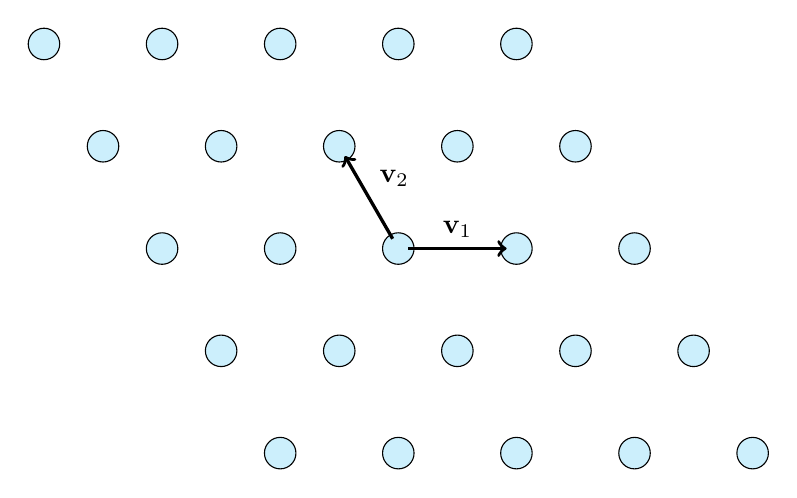
\begin{tikzpicture}
\def\angle{30}
\foreach \x in {0,...,4} {
\foreach \y in {0,...,4} {
	\filldraw[fill=cyan!20] ($1.5*\x*(1,0)+1.5*\y*(-{sin(\angle)},{cos(\angle)})$) circle (0.2cm) node (n\x\y) {}; 
}
}
\draw[->,very thick] (n22) to node[auto,swap] {$\mathbf v_2$} (n23) {};
\draw[->,very thick] (n22) to node[auto] {$\mathbf v_1$} (n32) {};
\end{tikzpicture}
\caption{A 2-dimensional Bravais lattice}
\label{fig:lattice_basis}
\end{figure}

Figure \ref{fig:lattice_basis} shows a 2-dimensional lattice with basis vectors $\mathbf{v}_1$ and $\mathbf{v}_2$. Two Bravais lattices are considered equivalent if they are invariant under the same symmetry group. In 2 dimensions, there are 5 different Bravais lattices and in 3 dimensions, there are 14 \cite{kittel2005introduction}. The choice of a lattice basis for a certain Bravais lattice is not unique.
The Bravais lattice is invariant under translation by any of its basis vectors, meaning it is a periodic structure. 

Physical crystals also have an atomic basis consisting of a set of atoms and positions for these atoms. The atomic basis is repeated at each point on the underlying Bravais lattice and generates the physical crystal. 
A simple example is NaCl, which has a face-centred cubic Bravais lattice, and a 2 atom atomic basis (shown in figure \ref{fig:nacl_lattice}).
\begin{figure}[t!]
    \centering
    \subfloat[NaCl basis atoms]{
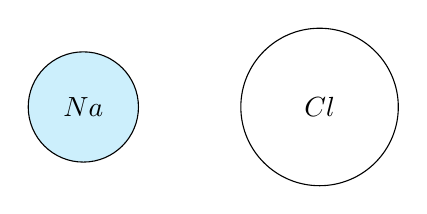
\begin{tikzpicture}
\filldraw[fill=cyan!20] (0, 0) circle (0.7cm) node {$Na$};
\filldraw[fill=white] (3, 0) circle (1cm) node {$Cl$};
\end{tikzpicture}
    }\qquad
    \subfloat[NaCl crystal cross-section showing two of three basis vectors]{
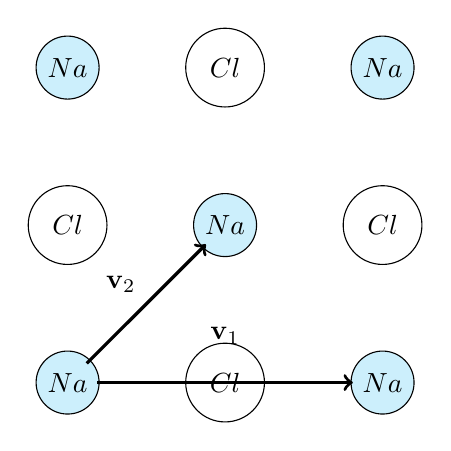
\begin{tikzpicture}
\foreach \x in {0, 2} {
	\foreach \y in {0,2} {
\filldraw[fill=cyan!20] ($(0, 0)+2*(\x, \y)$) circle (0.4cm) node (n\x\y) {$Na$};
}}
\filldraw[fill=cyan!20] ($(0, 0)+2*(1, 1)$) circle (0.4cm) node (n11) {$Na$};
\filldraw[fill=white] (2, 0) circle (0.5cm) node {$Cl$};
\filldraw[fill=white] (0, 2) circle (0.5cm) node {$Cl$};
\filldraw[fill=white] (2, 4) circle (0.5cm) node {$Cl$};
\filldraw[fill=white] (4, 2) circle (0.5cm) node {$Cl$};
\draw[->,very thick] (n00) to node[auto] {$\mathbf v_2$} (n11);
\draw[->,very thick] (n00) to node[auto,above=1em] {$\mathbf v_1$} (n20);
\end{tikzpicture}
    }\qquad
    \caption{NaCl atomic basis and crystal cross-section}
\label{fig:nacl_lattice}
\end{figure}
\subsubsection{The Unit Cell}
The unit cell is the set of points spanned by the lattice basis vectors, and is the repeating unit that the whole crystal is tiled up from (by translating it along all lattice vectors). Specifically, it is the set of points:
\begin{equation}\label{eq:unit_cell}
	\left\{\sum _{i=1}^n a_i \mathbf v_i \Big| a_i \in \mathbb{R}, 0<a_i<1, \mathbf{v}_i \in \mathcal V \right\}
\end{equation}
The volume of the unit cell is given by the determinant of the matrix made from placing its column basis vectors together:
\begin{equation}
	V = \det [\mathbf{v}_1 \mathbf{v}_2 ... \mathbf{v}_n]
\end{equation}
\subsubsection{Dual Lattice}
With every real lattice, we can associate a dual lattice in reciprocal space with basis vectors:
\begin{equation}\label{eq:dual_basis}
	\mathcal{W} = \{\vec{\omega}_1, \vec \omega _2, ..., \vec{\omega}_n\}
\end{equation}
And a set of dual lattice points:
\begin{equation}\label{eq:dual_lattice}
	\mathcal{G} = \left \{\sum_{i=1}^n a_i\vec{\omega}_i \Big | a_i \in \mathbb{Z}, \vec{\omega}_i \in \mathcal{W}  \right \}
\end{equation}
The real and dual bases have the property:
\begin{equation}
	\mathbf v _ i \cdot \vec\omega_j = 2\pi\delta_{ij}
\end{equation}
Due to the fact that the Bravais lattice is periodic, any observable will be periodic as well (For example, the electron density, $\rho(\mathbf{r})$\ ).

Since these observables will be periodic we have:
\begin{equation}\label{eq:periodic_observable}
	f(\mathbf r) = f(\mathbf r + \mathbf B) \text{ where } \mathbf B \in \mathcal B
\end{equation}
We can consider the fourier expansion of this function:
\begin{equation}\label{eq:f_fourier_expansion}
	f(\mathbf r + \mathbf B) = \sum_k f_k e ^ {i \mathbf G_k\cdot(\mathbf r + \mathbf B)} 
	= \sum _k f_k e ^ {i \mathbf G_k \cdot \mathbf r} e ^ {i \mathbf G_k \cdot \mathbf B}
\end{equation}
Where $\mathbf G_k \in \mathcal G$, $\sum_k$ is the sum over all vectors in $\mathcal G$ and the fourier component $f_k$ is given by:
\begin{equation}
	f_k = \frac{1}{V}\int_Cd\mathbf rf(\mathbf r)e^{-i\mathbf G_k\cdot \mathbf r}
\end{equation}
$C$ being the unit cell, and $V$ its volume.

Since equation \ref{eq:f_fourier_expansion} is true for $\mathbf{B} = \mathbf{0}$, this must mean that $e^{i\mathbf G_k\cdot \mathbf B_n} = 1$, $\forall k, n \in \mathbb{Z} $ and we have that $\mathbf G_k \cdot \mathbf B_n = 2\pi N$, $N\in \mathbb{Z}$. We can generate the dual lattice vectors from the real lattice vectors (using column-vectors for the real basis and row-vectors for the dual basis): 
\begin{gather}
	\vec{\omega}_i\cdot \mathbf{v}_j = 2\pi\delta_{ij} \\
	\begin{bmatrix} 
		\vec{\omega}_1 \\
		\vec{\omega}_2 \\
		\vdots \\
		\vec{\omega}_n \\
	\end{bmatrix}
	\begin{bmatrix}
		\mathbf{v}_1
		\mathbf{v}_2
		...
		\mathbf{v}_n
	\end{bmatrix} = 2\pi
	\begin{bmatrix}
		1 & 0  & ... & 0 \\
		0 & 1 &  ... & 0  \\
		\vdots & \vdots & \ddots & \vdots \\
		0 & 0 & \hdots & 1 
	\end{bmatrix}
	\\
	\begin{bmatrix} 
		\vec{\omega}_1 \\
		\vec{\omega}_2 \\
		\vdots \\
		\vec{\omega}_n \\
	\end{bmatrix}
	= 2\pi
	\begin{bmatrix}
		\mathbf{v}_1
		\mathbf{v}_2
		...
		\mathbf{v}_n
	\end{bmatrix} ^{-1}
\end{gather}
Since the lattices are related to each other through a fourier transform, the dual lattice to the dual lattice is the original lattice.
In 3 dimensions, the reciprocal lattice of the simple cubic lattice is the simple cubic lattice 
(with each vector having a reciprocal length), the reciprocal lattice of the FCC lattice is BCC, and vice versa.
\subsubsection{Bloch's Theorem}
The periodicity of the lattice leads to a constraint on the wavefunction of electrons in the crystal:
\begin{equation}\label{eq:bloch_wave}
	\psi_\mathbf k(\mathbf r) = e^{i\mathbf{k}\cdot \mathbf{r}}u_\mathbf k(\mathbf r)
\end{equation}
Where $u_\mathbf k(\mathbf r)$ has the same period as the crystal the wave is in.
We can prove this using the translation operator $\hat T_\mathbf B$ where $\hat T_\mathbf B f(\mathbf r) = f(\mathbf r + \mathbf B)$, and $\mathbf B$ is some lattice vector. Let $\psi_\mathbf k(\mathbf r)$ be an eigenstate of the translation operator:
\begin{equation}
	\hat T_\mathbf B \psi_\mathbf k(\mathbf r) = A \psi_\mathbf k(\mathbf r)
\end{equation}
Since the state is normalised to unity, we can write $A=e^{i\mathbf k \cdot \mathbf B}$. If we define another function, $u_\mathbf k(\mathbf r) = e^{-i\mathbf k \cdot \mathbf r}\psi_\mathbf k(\mathbf r)$ and then operate on it with the lattice translation operator:
\begin{equation}\label{eq:bloch_proof}
\hat T_\mathbf B u_\mathbf k(\mathbf r) = u_\mathbf k(\mathbf r + \mathbf B) = 
e^{-i\mathbf k \cdot \mathbf r}e^{-i\mathbf k \cdot \mathbf B} \psi_\mathbf k(\mathbf r + \mathbf B) = 
e^{-i\mathbf k \cdot \mathbf r}e^{i\mathbf k \cdot (\mathbf B - \mathbf B)} \psi_\mathbf k(\mathbf r) = u_\mathbf k(\mathbf r)
\end{equation}
Which shows that $u_\mathbf k(\mathbf r)$ has the same periodicity as the lattice. The relation $u_\mathbf k(\mathbf r) = e^{-i \mathbf k \cdot \mathbf r}\psi_\mathbf k(\mathbf r)$ is then inverted to get the result in equation \ref{eq:bloch_wave}.
\subsubsection{Phonons}

The nuclei in a lattice are not completely static, and in fact their ability to move is an important factor in observables of the crystal, like heat capacity and thermal expansion. We can model the nuclei as chains of harmonic oscillators, interacting with their nearest neighbours, and find solutions to the displacements of the nuclei as monochromatic plane waves \cite{landau1980statistical}:
\begin{equation}
	\mathbf u(\mathbf n) = \mathbf e(\mathbf k) \exp{[i(\mathbf k \cdot \mathbf r_n - \omega t)]}
\end{equation}
Where $\mathbf n$ is the label of some atom, $\mathbf r_n$ is the position of that atom and $\mathbf e(\mathbf k)$ is the polarisation vector and amplitude of the wave. In 3 dimensions, if $\mathbf e(\mathbf k)$ points in the direction of $\mathbf k$ the wave is longitudinal, and if it is perpendicular then the wave is transverse.

In the quantum view, the phonons are goldstone bosons: massless particles which carry quanta of energy through the lattice. We get the free energy:
\begin{equation}
	F(T, V) = N\epsilon_0 + TV\sum_{\alpha=1}^{3\nu}\int \ln \left[ 1-\exp\left(-\frac{\hbar \omega_\alpha(\mathbf k)}{T}\right)\right]g_\alpha(\omega)d\omega
\end{equation}

\begin{figure}
\centering
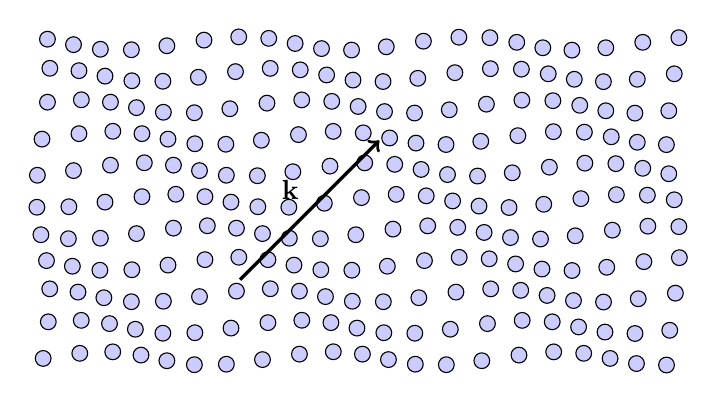
\begin{tikzpicture}
\tikzmath{
int \px;
\a = 0.3;
\s = 0.4;
\kx = 50;
\ky = 50;
\kmag = sqrt((\kx)^2+(\ky)^2);
\ukx = \kx/\kmag;
\uky = \ky/\kmag;
for \px in {0,...,20}{
for \py in {0,...,10}{
\dx=\a*sin(\px*\kx+\py*\ky)*\ukx;
\dy=\a*sin(\px*\kx+\py*\ky)*\uky;
\vx = \s*(\px+\dx);
\vy = \s*(\py+\dy);
{
	\filldraw[fill=blue!20] (\vx, \vy) circle (0.1cm) node (n\px\py) {};
};};
};
{\draw[->,very thick] (2.5, 1) to node[auto] {$\mathbf k$} (2.5+\ukx/\s, 1+\uky/\s);};
}
\end{tikzpicture}
\label{fig:phonon:disturbance}
\caption{A longitudinal phonon with wave-vector $\mathbf k$ in a 2-dimensional lattice}
\end{figure}

\subsection{Density Functional Theory}
\subsubsection{The Thomas-Fermi Model}
The first attempt to determine the distribution of electrons, the density $n(\mathbf r)$, in an atom using the newly developed quantum theory was made simultaneously in 1927 by Llewellyn Thomas \cite{thomas_1927} and Enrico Fermi \cite{fermi1927metodo}. This method provides a method to approximately calculate the energy of some atomic structure, in the form of a functional for the electron density:
\begin{equation}\label{eq:thomas-fermi}
	E[n(\mathbf r)] = \frac{3}{10}(3\pi^2)^{\frac{2}{3}}\int n^{\frac{5}{3}}(\mathbf r) d \mathbf r + \frac{1}{2}\int\int\frac{n(\mathbf r_1) n(\mathbf r_2)}{\left| \mathbf r_1 - \mathbf r_2\right|}d\mathbf r_1 d\mathbf r_2 + \int v_{ext}(\mathbf r) n(\mathbf r) d \mathbf r + E_{nn}
\end{equation}
Where the first term is the kinetic contribution, the second is the electron charge density self-interaction, the third is the electron's interaction with the external system and the fourth is the energy contained in the atomic nuclei/other elements of the system.

This model has a few large problems: the derivative of the energy when increasing the electron number is continuous; there is no electronic shell structure; and it doesn't predict binding \cite{lieb1977thomas}. This would be improved upon by the Hohenberg-Kohn theorems, which would give a strong theoretical backing to the problem of finding these densities.

\subsubsection{The Hohenberg-Kohn Theorems}
The Hohenberg-Kohn theorems \cite{PhysRev.136.B864} are two theorems, developed in 1964 by Pierre Hohenberg and Walter Kohn, which are the backing to modern density functional theory (DFT). These theorems relate some given external potential of an atomic system to the ground state charge density that the mobile charged particles will adopt. They are stated as \cite{martin_2004}:
\begin{displayquote}
	\textbf{Theorem I}: For any system of interacting particles in an external potential $v_\mathrm{ext}(\mathbf r)$, the potential $v_\mathrm{ext}(\mathbf r)$ is determined uniquely, except for a constant, by the ground state particle density $n_0(\mathbf{r})$.
\\
	\textbf{Theorem II}: A \textit{universal functional} for the energy $E[n]$ in terms of the density $n(\mathbf r)$ can be defined, valid for any external potential $v_\mathrm{ext}(\mathbf r)$.
For any particular $V_\mathrm{ext}(\mathbf r)$, the exact ground state energy of the system is the global minimum value of this functional, and the density $n(\mathbf r)$ that minimises the functional is the exact ground state density $n_0(\mathbf r)$.
\end{displayquote}
The proofs to these theorems are relatively simple, making use of the quantum variational principle \cite{shankar2012principles}. We need to make a restriction though, that the ground state of the hamiltonians in the proofs are non-degenerate.
To prove the first theorem, we use proof by contradiction with two different hamiltonians $\hat H_1, \hat H_2$ with ground state wavefunctions $\ket{\psi_1}, \ket{\psi_2}$ which give the respective ground state energies $E^0_n=\braket{\psi_n | \hat H_n | \psi_n}$. 
The hamiltonians can be separated into:
\begin{equation}
\hat H_n = \hat F_{HK} + \hat V_{n, \mathrm{ext}}
\end{equation}
Where $\hat F_{HK}$ contains the electron kinetic energy operator, and the electron-electron interaction operator, and is the same for the different hamiltonians. The potential operator $\hat V_{n, \mathrm{ext}}$ contains the information of the external potential on the electrons (caused by the nuclei, and maybe other factors).
We then pose that the two different potentials in the hamiltonians give rise to the same ground-state electronic density $n_0(\mathbf r)$.
The energy of the system can also be written as a functional of the electron density as:
\begin{equation}\label{eq:energy_functional}
E[n(\mathbf r)] = F_{HK}[n(\mathbf r)]+ \int n(\mathbf r)v_{\mathrm{ext}}(\mathbf r)d\mathbf r
\end{equation}
Where $F[n(\mathbf r)]$ contains the electron kinetic energy and the electron-electron interaction energy, and $v_{\mathrm{ext}}(\mathbf r)$ is the external potential.
Using the variational principle, we have:
\begin{equation} 
	E^0_1 < \braket{\psi_2 | \hat H_1 | \psi_2} = \braket{\psi_2 | \hat H_2 | \psi_2} + \braket{\psi_2 |\hat H_1 - \hat H_2 |\psi_2}
\end{equation}
Using the energy functional from equation \ref{eq:energy_functional}, we can rewrite this as:
\begin{equation}\label{eq:contra_1}
E^0_1 - E^0_2 < \int n_0(\mathbf r)(v_{1,\mathrm{ext}}(\mathbf r)-v_{2,\mathrm{ext}}(\mathbf r)) d\mathbf r
\end{equation}
Swapping the indices, and rearranging gives:
\begin{equation}
E^0_1 - E^0_2 > \int n_0(\mathbf r)(v_{1,\mathrm{ext}}(\mathbf r)-v_{2,\mathrm{ext}}(\mathbf r)) d\mathbf r
\end{equation}
These equations are in contradiction with each other, and therefore, up to an additive constant, the external potential must be determined uniquely by the ground state electron density and vice versa.

To prove the second theorem, we use an energy functional $E[n(\mathbf r)]$, with some external potential $v_{\mathrm{ext}}$ that is minimised by a density $n_1(\mathbf r)$ and we consider some different density $n_2(\mathbf r)$. 
By the first theorem, the wavefunctions determined by these densities must be different ($\ket{\psi_1}, \ket{\psi_2}$) and so, using the variational principle we have:
\begin{equation}\label{eq:hk_2}
E_1 = \braket{\psi_1 | \hat H _1 | \psi_1} < \braket{\psi_2 | \hat H _1 | \psi_2} = E_2
\end{equation}
So the energy functional is minimised by this ground state density.

The Hohenberg-Kohn theorems presented in this way rely on what are called $v$-representable densities. The minimisation of the energy in theorem II is perfomed over the set of densities that arise from some external potential $v_{ext}$, hence $v$-representable. There is a larger set of densities: the $N$-representable densities, which is defined as the set of all densities which integrate to $N$, the number of charges in your Schrodinger equation.

To find the density with the Hohenberg-Kohn approach, we minimise the total energy functional $E[n(\mathbf r)]$ over the set of $v$-representable densities. A problem with this is that the set of $v$-representable densities is not explicitly known \cite{GONIS201623}; it is not possible to know whether some given $n(\mathbf r)$ is a density corresponding to a potential $v_{ext}(\mathbf r)$.

\subsubsection{Constrained Search}
There is another method to find the electron density which is due to Mel Levy \cite{Levy6062} and Elliott Lieb \cite{lieb1985density}. This formulation sidesteps the problem of $v$-representability by instead considering the $N$-representable densities.
We write down the total energy of the quantum system as a functional of the charge density of the system:
\begin{equation}
	E[n(\mathbf r)] = \braket{\Psi|\hat T + \hat V_{ee}|\Psi} + \int n(\mathbf r)v_{ext}(\mathbf r)d\mathbf r + E_{nn}
\end{equation}
Where $\hat V_{ee}$ is the potential due to the charge density and $E_{nn}$ is the energy from elements of the system that aren't electrons (eg. the nuclei). 
We now consider the set of wavefunctions $\left\{\ket{\Psi}\right\}$ which reproduce the given electron density $n(\mathbf r)=\int \braket{\Psi|\Psi}d\mathbf{r_2}\mathellipsis d\mathbf{r_n}$, and understand that the energy of the system with this density will be the minimum value of the energies given by the set $\left\{\ket{\Psi}\right\}$:
\begin{equation}
\begin{split}
E[n(\mathbf r)] = \min_{\ket{\Psi} \rightarrow n(\mathbf r)}\left\{\braket{\Psi | \hat T + \hat V_{ee} | \Psi}\right\} + \int n(\mathbf r) v_{ext}(\mathbf r) d \mathbf r + E_{nn}\\
E[n(\mathbf r)] = F_{LL}[n(\mathbf r)] + \int n(\mathbf r) v_{ext}(\mathbf r) d\mathbf r + E_{nn}
\end{split}
\end{equation}
Where the Levy-Lieb energy functional $F_{LL}[n(\mathbf r)]$ contains the minimisation over the wavefunctions reproducing $n(\mathbf r)$.
To find the correct energy density, a minimisation is then performed over all $N$-representable densities:
\begin{equation}\label{eq:levylieb}
 E_0 = \min_{n(\mathbf r)} \left\{ F_{LL}[n(\mathbf r)] + \int n(\mathbf r) v_{ext}(\mathbf r) d \mathbf r\right\} + E_{nn}
\end{equation}
This formulation of the search for the correct density changes the search from the unknown domain of $v$-representable densities to the known domain of $N$-representable densities and also allows us to search in systems with degenerate ground states. 

The Hohenberg-Kohn theorems and the Levy-Lieb constrained search give us a theoretical way to find the correct density for a system, but two large questions still remain: 
\begin{displayquote}
\textbf{1:} How do we practically perform the minimisation?

\textbf{2:} What form does the energy functional $F[n(\mathbf r)]$ take?
\end{displayquote}
\subsubsection{Kohn-Sham Equations}
Practically, performing the search over all general $N$-representable states is a tough task, we need something to guide us. 
This comes in the form of the Kohn-Sham equations \cite{kohn1965self}, developed in 1965 by Lu Jeu Sham and Walter Kohn, the year after the H-K theorems were determined. 
These equations change the problem of solving the Schrodinger equation for many electrons into solving it for a set of non-interacting orbitals $\{\phi_i\}$. This is derived by considering variations in the energy with respect to the orbitals, with the constraint that $n(\mathbf r) = \sum \phi^*(\mathbf r)\phi(\mathbf r)$.

The Kohn-Sham equations for the non-interacting orbitals are:
\begin{equation}\label{eq:kohn-sham}
\left(-\frac{\hbar^2}{2m}\nabla^2 + v_{KS}(\mathbf r)\right)\phi_i(\mathbf r) = \epsilon_i \phi_i(\mathbf r)
\end{equation}
Where the Kohn-Sham potential $v_{KS}(\mathbf r)$ is defined as:
\begin{equation}\label{eq:kohn-shampotential}
v_{KS}(\mathbf r) = v_{ext}(\mathbf r) + \int \frac{n(\mathbf r')}{\left|\mathbf r - \mathbf {r'}\right|}d\mathbf {r'} + v_{xc}(\mathbf r)
\end{equation}
The sum of the external potential, the classical electron self-interaction, and an exchange correlation term coming from quantum effects on the electrons. 
\begin{figure}
\centering
	\tikzstyle{decision} = [diamond, draw, fill=blue!20, 
    text width=4.5em, text badly centered, node distance=3cm, inner sep=0pt]
\tikzstyle{block} = [rectangle, draw, fill=blue!20, 
    text width=6em, text centered, rounded corners, minimum height=4em]
\tikzstyle{line} = [draw, -latex']
\tikzstyle{cloud} = [draw, ellipse,fill=red!20, node distance=3cm,
    minimum height=2em]
    
\begin{tikzpicture}[node distance = 4cm, auto]
    % Place nodes
    {\node [block] (init) {initial guess at charge density $n(\mathbf r)$};}
    {\node [block, right of=init] (potential) {calculate new $v_{KS}(\mathbf r)$ from $n(\mathbf r)$};}
    {\node [block, right of=potential] (update) {solve Kohn-Sham equations for new $n(\mathbf r)=\sum_i \phi^*_i\phi_i$};}
    {\node [decision, below of=update, node distance = 4cm] (decide) {are convergence criteria met?};}
    {\node [block, right of=decide] (stop) {output converged charge density};}
    
    {\path [line] (init) -- (potential);}
    {\path [line] (potential) -- (update);}
    {\path [line] (update) -- (decide);}
    {\path [line] (decide) -- node {yes} (stop);}
    {\path [line] (decide) -| node {no}(potential);}
\end{tikzpicture}
\caption{The process of self-consistently solving the Kohn-Sham equations for the charge density}
\end{figure}

The Kohn-Sham equations are exact (bar relativity), with the limitation coming from the fact that we don't have an exact form for the exchange correlation potential. 
If this was known, we would be able to recreate any system's electron density to the precision allowed by our computers.

\subsubsection{Density Functional Perturbation Theory}

\section{Methods}
All density functional theory were performed using the Quantum Espresso software \cite{0953-8984-21-39-395502}, and data analysis was performed using python.

Ultrasoft pseudopotentials were chosen for the three different elements from the GBRV pseudopotential website \cite{rutgers} and the Standard Solid State Pseudopotential library (SSSP) \cite{SSSPwebsite}. 
These are shown in table \ref{tab:pseudopotentials}.
\begin{table}
\centering
	\begin{tabular}{|c|c|}
\hline
Element & Pseudopotential \\
\hline
Silicon & si\_pbe\_v1.uspp.F.UPF \cite{rutgers} \\
Tin & sn\_pbe\_v1.4.uspp.F.UPF \cite{rutgers} \\
Sodium & Na\_pbe\_v1.uspp.F.UPF \cite{SSSPwebsite} \\
\hline
\end{tabular}
\caption{Pesudopotentials used}
\label{tab:pseudopotentials}
\end{table}

Ultrasoft potentials were chosen because of their fast convergence with wavefunction cutoff compared to norm-conserving potentials \cite{vanderbilt1990soft}. 

The calculations for silicon and tin were performed on the James Clerk Maxwell building computing clusters, and the calculations for sodium were performed on the ARCHER supercomputer \cite{archer}.

For each structure, calculations were performed first to check the dependence of the pseudopotentials on the plane wave cutoff, ecutwfc. This was done by calculating the energy and the pressure at different ecutwfc values, and taking the difference in energy/pressure at each point with the energy/pressure at the highest calculated ecutwfc. This last value is set high enough to assume it is ``converged''. 
The charge density and potential cutoff ecutrho was set to $8\times$ ecutwfc as the pseudopotentials were ultrasoft, non conserving potentials.

\begin{figure}
	\centering
	\subfloat{
		\includesvg[width=0.4\textwidth]{./figures/silicon_convergence_e_ecut.svg}
}\qquad
\subfloat{
		\includesvg[width=0.4\textwidth]{./figures/silicon_convergence_p_ecut.svg}
}\qquad
\caption{Silicon energy and pressure convergence vs ecutwfc}
\label{fig:silicon_ecut_convergence}
\end{figure}
\begin{figure}
	\centering
	\subfloat{
		\includesvg[width=0.4\textwidth]{./figures/tin_convergence_e_ecut.svg}
}\qquad
\subfloat{
		\includesvg[width=0.4\textwidth]{./figures/tin_convergence_p_ecut.svg}
}\qquad
\caption{Tin energy and pressure convergence vs ecutwfc}
\label{fig:tin_ecut_convergence}
\end{figure}
\begin{figure}
	\centering
	\subfloat{
		\includesvg[width=0.4\textwidth]{./figures/sodium_convergence_e_ecut.svg}
}\qquad
\subfloat{
		\includesvg[width=0.4\textwidth]{./figures/sodium_convergence_p_ecut.svg}
}\qquad
\caption{Sodium energy and pressure convergence vs ecutwfc}
\label{fig:sodium_ecut_convergence}
\end{figure}

Figures \ref{fig:silicon_ecut_convergence} to \ref{fig:sodium_ecut_convergence} shows the convergence of energy and pressure for each of the different pseudopotentials used.
The ecuts chosen for each element are shown in table \ref{tab:chosenecuts}.

\begin{table}
\centering
	\begin{tabular}{|c|c|}
\hline
Element & chosen ecutwfc (Ry)\\
\hline
Silicon &  30\\
Tin &  50\\
Sodium &  40\\
\hline
\end{tabular}
\caption{Chosen ecutwfc values for the different elements}
\label{tab:chosenecuts}
\end{table}

The next step was to check the convergence of each element with the k-points grid. The convergence tests were performed for diamond cubic silicon, $\alpha$-tin, and face-centred cubic (FCC) sodium. For these convergence tests, the differences in energy and pressure from a ``converged'' reference point were again tested against a changing k-grid resolution. This grid had a resolution $k\times k \times k$ for all three elements.

\begin{figure}
	\centering
	\subfloat{
		\includesvg[width=0.4\textwidth]{./figures/silicon_convergence_e_k.svg}
}\qquad
\subfloat{
		\includesvg[width=0.4\textwidth]{./figures/silicon_convergence_p_k.svg}
}\qquad
\caption{Silicon energy and pressure convergence vs k-grid}
\label{fig:silicon_k_convergence}
\end{figure}
\begin{figure}
	\centering
	\subfloat{
		\includesvg[width=0.4\textwidth]{./figures/tin_convergence_e_k.svg}
}\qquad
\subfloat{
		\includesvg[width=0.4\textwidth]{./figures/tin_convergence_p_k.svg}
}\qquad
\caption{Tin energy and pressure convergence vs k-grid}
\label{fig:tin_k_convergence}
\end{figure}
\begin{figure}
	\centering
	\subfloat{
		\includesvg[width=0.4\textwidth]{./figures/sodium_convergence_e_k.svg}
}\qquad
\subfloat{
		\includesvg[width=0.4\textwidth]{./figures/sodium_convergence_p_k.svg}
}\qquad
\caption{Sodium energy and pressure convergence vs k-grid}
\label{fig:sodium_k_convergence}
\end{figure}

From these convergences the k-grids for each element were chosen, and the k-grids for the different structures of each element were chosen to have as similar as possible sampling in k-space. The chosen k-grids and their offsets are shown in table \ref{tab:k-grids}.

\begin{table}
	\centering
	\begin{tabular}{|c|c|c|}
		\hline
		Structure & k-grid & k-grid offset \\
		\hline
		Diamond cell silicon & $(12, 12, 12)$ & $(1, 1, 1)$ \\
		$\alpha$-tin & $(16, 16, 16)$ & $(1, 1, 1)$ \\
		$\beta$-tin & $(12, 12, 20)$ & $(1, 1, 1)$ \\
		FCC sodium & $(20, 20, 20)$ & $(1, 1, 1)$ \\
		BCC sodium & $(20, 20, 20)$ & $(1, 1, 1)$ \\
		9R sodium & $(20, 20, 20)$ & $(1, 1, 1)$ \\
		\hline
	\end{tabular}
	\caption{Structure SCF k-grids and offsets}
	\label{tab:k-grids}
\end{table}

The SCF calculations for $\alpha$ and $\beta$-tin and FCC, BCC and 9R sodium were performed using Marzari-Vanderbilt cold smearing \cite{marzari1999thermal} with a smearing width of $0.02$ Ry, as they are not insulators. 
The $\alpha$-tin and $\beta$-tin structures were calculated at their $T=0K$ equilibrium volume. This was done by performing variable-cell relaxations on the structures targetting a pressure of $0$GPa. The calculations on silicon were performed over a linearly spaced range of lattice constants from 10.28 Bohr to 10.4 Bohr in steps of 12 Bohr. The sodium FCC calculations were performed over a lattice constant range of 8.65 Bohr to 10.28 Bohr with 16 different points. The sodium BCC calculations were performed over a lattice constant range of 6.88 Bohr to 8.4 Bohr with 18 different points. The 9R sodium structure was relaxed to 0GPa. The scf and variable-cell relaxation calculations were all performed with the pw.x tool from Quantum Espresso. For all structures the scf convergence threshold (conv\_thr) was set to \num{1e-10} Ry.

The density functional perturbation calculations were performed with the Quantum Espresso ph.x tool. Silicon and the sodium structures were calculated with q-grids of $6\times 6\times 6$, with the exception of 9R which was calculated with a q-grid of $4\times4\times4$ and the two tin allotropes were calculated with an $8\times8\times8$ q-grid. A self-consistency threshold of \num{1e-16} (tr2\_ph) was set for all calculations.

After a full set of phonon perturbations was calculated for each structure, these were Fourier transformed into the force constants matrix using the quantum espresso tool q2r.x. The matdyn.x tool was then used to create the band structure and density of states of the different structures. One the density of states $g(\omega)$ is obtained, the free energy phonon contribution can be calculated. This done by the Quantum Espresso fqha.x tool, which performs the integral:
\begin{equation}
	\label{eq:phononfreeenergy}
	F(V, T) = \int_0^\infty \left[\frac{\hbar\omega}{2} + k_bT \ln\left(1-\exp\left\{\frac{\hbar \omega}{k_bT}\right\} \right) \right]g_V(\omega) d\omega
\end{equation}
Where $g_V(\omega)$ is the density of states at the volume $V$. The free energy can then be written as the sum of the contribution from the electrons and the phonons: 
\begin{equation}\label{eq:total_free_energy}
F(V, T) = F_{scf}(V)|_{T=0} + F_{phon}(V, T)
\end{equation}

This is then transformed into the Gibb's free energy potential using a Legendre transform from volume to pressure. The free energy $F(V)|_T$ at each temperature was fit to an empirical equation of state, $E(V)$, and the pressure $P(V)$ was recovered as $-\frac{\partial E(V)}{\partial V}$. The legendre transform is then:
\begin{equation}
	G(T, P) = PV(P) + F(T, V(P))
\end{equation}
For each of the different materials compared, the free energy surfaces were overlaid on the same coordinates, and the minimum surface at each point gives the preferred structure. The intersections of the surfaces give the transition curves.

Silicon's energy was fitted with the Vinet equation of state:
\begin{equation}\label{eq:vinet}
E(\eta) = E_0 + \frac{4B_0V_0}{(B'_0-1)^2} + \frac{2B_0V_0}{(B'_0-1)^2}\exp{\left(\frac{3}{2}(B'_0-1)(1-\eta)\right)}[3(B'_0-1)(1-\eta)-2]
\end{equation}
Sodium's energy was fitted to the Murnaghan equation of state:
\begin{equation}\label{eq:bm}
E(\eta) = E_0+\frac{B_0V_0}{B'_0}\eta^3\left( \frac{\eta^{-3B'_0}}{B'_0-1}+1\right)-\frac{B_0V_0}{B'_0-1}
\end{equation}
Where, for both $\eta=\frac{V}{V_0}$, $E_0$ is the equilibrium energy, $V_0$ is the equilibrium volume, and $B_0, B'_0$ are the equilibrium bulk modulus and the bulk modulus pressure derivative respectively.

The fitting of the Vinet equation for silicon was done with SciPy's curve\_fit function \cite{scipy}, and the fitting for sodium was performed with Quantum Espresso's ev.x tool. The ev.x tool outputs a list of pressures for each volume input, so the irregular grid of points $G(T, P)$ was interpolated using SciPy's griddata function.
\section{Results and Discussion}
\subsection{Pseudopotential Convergence}
\subsection{Silicon}
\begin{figure}
	\centering
	\subfloat[Silicon lattice parameter fit vs temperature]{
		\includesvg[width=0.4\textwidth]{./figures/si_latparam_temp.svg}\label{fig:silicon_lat_fit}
}\qquad
\subfloat[Silicon lattice parameter fit residuals vs temperature]{
	\includesvg[width=0.4\textwidth]{./figures/si_latparam_residuals.svg}\label{fig:silicon_fit_residuals}
	}\qquad
\end{figure}

\begin{figure}
	\centering
	\includesvg[width=0.8\textwidth]{./figures/si_band_structure.svg}
	\label{fig:si_band_structure}
	\caption{Silicon calculated phonon band structure}
\end{figure}

\begin{figure}
	\centering
	\includesvg[width=0.8\textwidth]{./figures/si_thermal_expansion.svg}
	\label{fig:si_thermal_expansion}
	\caption{Fitted linear thermal expansion coefficient of silicon vs experimental data \cite{middelmann2015thermal}}
\end{figure}
\subsection{Tin}
\begin{figure}
	\centering
	\subfloat{
		\includesvg[width=0.4\textwidth]{./figures/tin_convergence_e_k.svg}
}\qquad
\subfloat{
		\includesvg[width=0.4\textwidth]{./figures/tin_convergence_p_k.svg}
}\qquad
\end{figure}
\begin{figure}
	\centering
	\includesvg[width=0.8\textwidth]{./figures/tin_transition_temperature.svg}
	\label{fig:sn_transition}
	\caption{Transition between $\alpha$ and $\beta$ tin}
\end{figure}
\subsection{Sodium}
\begin{figure}
	\centering
	\subfloat{
		\includesvg[width=0.4\textwidth]{./figures/sodium_convergence_e_k.svg}
}\qquad
\subfloat{
		\includesvg[width=0.4\textwidth]{./figures/sodium_convergence_p_k.svg}
}\qquad
\end{figure}
\begin{figure}
	\centering
	\includesvg[width=\textwidth]{./figures/sodium_pt_diagram.svg}
\end{figure}

\section{Conclusion}

\section{References}

% This command tells LaTeX how to format your references in the biblography. The standard plain formatting, with
% references appearing in the order they are cited, is absolutely fine for our needs.
\bibliographystyle{unsrt}

% This command includes the reference list. You will need to compile two or three times (perhaps BiBTeXing after
% the first time) to get the references in synch with the text.
\bibliography{ref}

% This command switches to appendices. The page count ends here.
% NOTE: the material contained in appendices will NOT count towards the assessment of your report.
% Consequently the main text should be self-contained.
\appendix

\end{document}
